\documentclass[9pt]{beamer}
%\usepackage{amsmath,amssymb,amsthm,tikz-cd}
\usetheme{Madrid}
\usecolortheme{default}
\DeclareMathOperator{\Hom}{Hom}
\DeclareMathOperator{\Det}{det}
\DeclareMathOperator{\supp}{supp}

\title[Differentiable manifolds and the Stokes' Theorem]
{Differentiable manifolds and the Stokes' Theorem}

\author[Jonathan Lau] % (optional)
{Jonathan Lau}

\AtBeginSection[]
{
	\begin{frame}
		\frametitle{Table of Contents}
		\tableofcontents[currentsection]
	\end{frame}
}

\begin{document}
	
\frame{\titlepage}

\begin{frame}
	\frametitle{Table of Contents}
	\tableofcontents
\end{frame}

\section{Manifolds}
	
\begin{frame}{Stokes' Theorem}
    Stokes' Theorem:\[\int_Md\omega = \int_{\partial M} \omega\]

    Special cases: \[\int_{\partial D} Pdx+Qdy = \int_D \left(\frac{\partial Q}{\partial x}-\frac{\partial P}{\partial y}\right) dA\]
    \[\int_{\partial V}  F\cdot dS = \int_V \text{div} F\]
\end{frame}

\begin{frame}{Upper Half Space}
    \begin{block}{}
        The upper half space is $\mathcal{H}^n=\{(x_1, \dots, x_n)\in \mathbb{R}^n\mid x_n \geq 0\}$. Its boundary is $\partial \mathcal{H}^n = \{(x_1, \dots, x_n)\in \mathbb{R}^n\mid x_n = 0\}$.
    \end{block}
    \begin{center}
        
        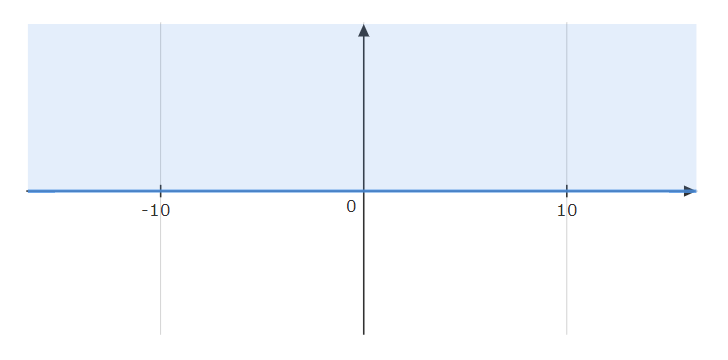
\includegraphics[scale=0.6]{upper_half.PNG}
    \end{center}

\end{frame}
\begin{frame}{Charts}

    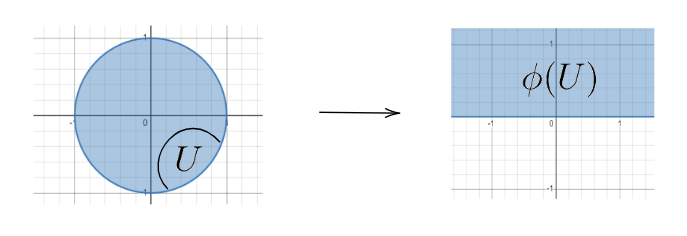
\includegraphics[scale=0.8]{chart.PNG}
    
\end{frame}

\begin{frame}{Manifolds}
    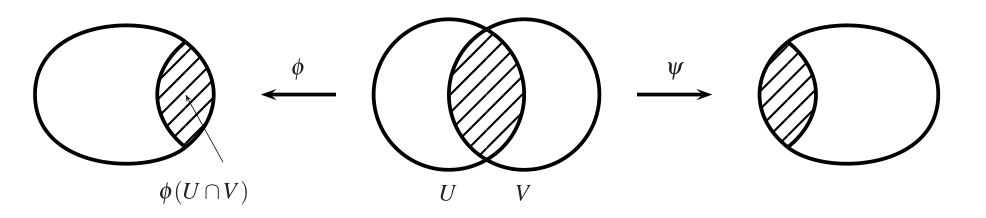
\includegraphics[scale=0.55]{compatible.PNG}

\end{frame}

\begin{frame}{Boundary}
    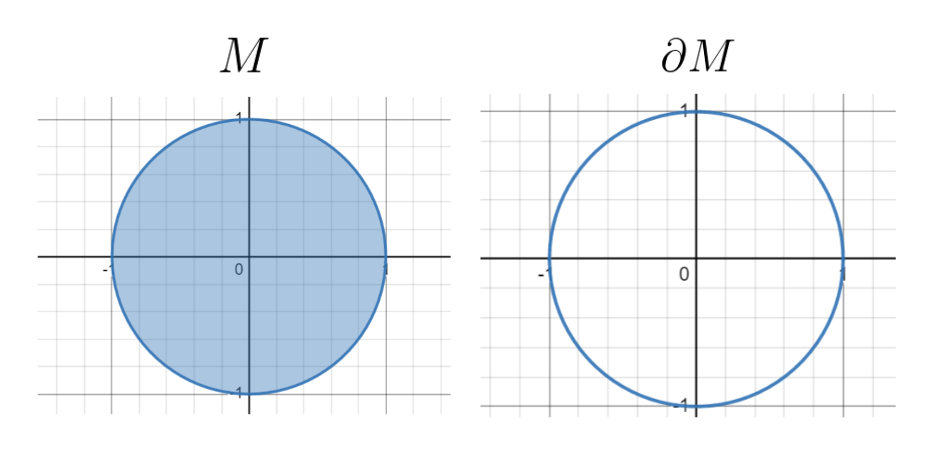
\includegraphics[scale=0.6]{boundary.PNG}
\end{frame}

\begin{frame}{Examples}
    \begin{center}  
    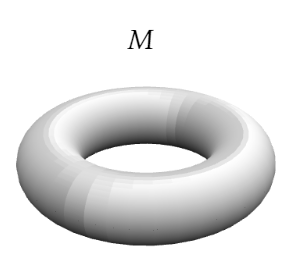
\includegraphics[scale=0.6]{torus.png}
    \end{center}
\end{frame}

\begin{frame}{Examples}
    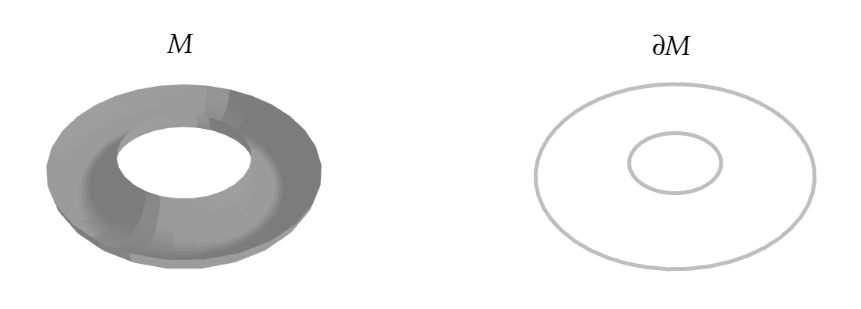
\includegraphics[scale=0.6]{torus1.PNG}
\end{frame}

\section{Tangent Space and differential forms}


\begin{frame}{Tangent Space}
    \begin{center}
        
    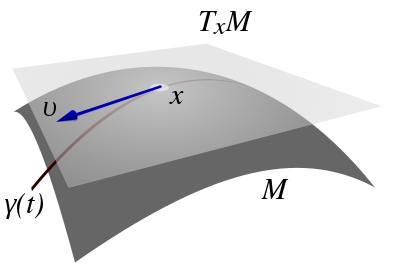
\includegraphics[scale=0.5]{tangent_space.png}
    \end{center}
\end{frame}

\begin{frame}{Tangent vectors}
\begin{center}
    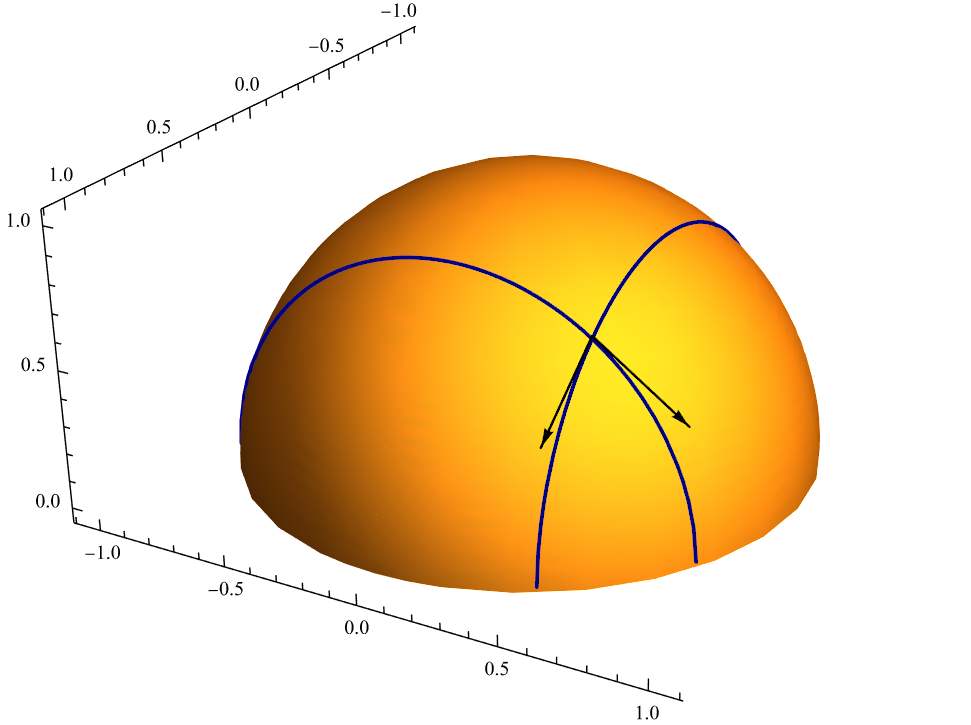
\includegraphics[scale=0.4]{uppersphere.png}
\end{center}
\end{frame}

\begin{frame}{Smooth Functions}
    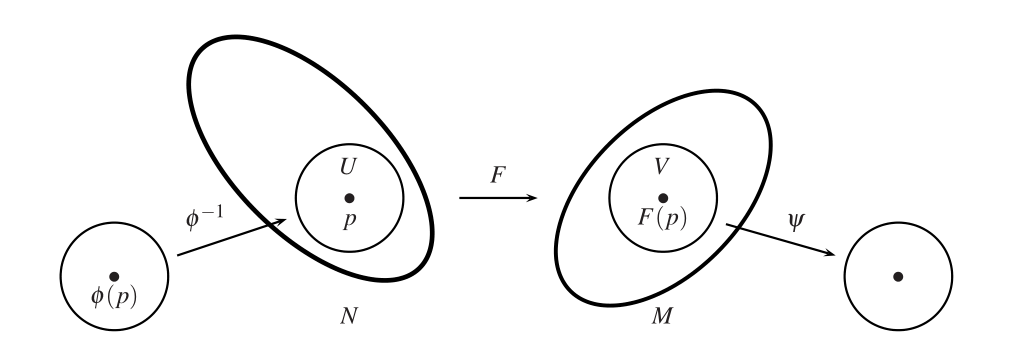
\includegraphics[scale=0.55]{smooth_function.PNG}
\end{frame}



\begin{frame}{Differential}

    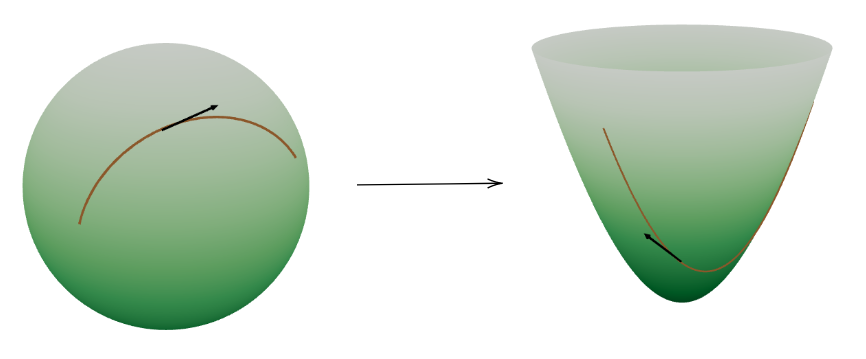
\includegraphics[scale=0.6]{differential.PNG}
\end{frame}

\begin{frame}{Alternating multilinear}
    \begin{center}
        Alternating:

        $\omega_p(v_1, \dots, v_i, v_{i+1}, \dots, v_k)=-\omega_p(v_1, \dots, v_{i+1}, v_1, \dots, v_k)$\\[15pt]

        Multilinear:

        $\omega_p(v_1, \dots,v_i+cw_i, \dots, v_k)=\omega_p(v_1, \dots,v_i, \dots, v_k)+c\omega_p(v_1, \dots,w_i, \dots, v_k)$
    \end{center}
\end{frame}

\section{Integration of Differential \texorpdfstring{$n$}{n}-Forms}

\begin{frame}
    \begin{block}{Partition of Unity}
        Let $\{(U_\alpha, \phi_\alpha)\}_{\alpha\in A}$ be an atlas on $M$. A partition of unity on a manifold $M$ is a collection of nonnegative smooth functions $\{\rho_\alpha:M \rightarrow \mathbb{R}\}_{\alpha\in A}$ such that \begin{enumerate}[i]
            \item the collection of supports, $\{\supp\rho_\alpha\}_{\alpha\in A}$, is locally finite,
            \item $\sum_{\alpha\in A} \rho_\alpha = 1.$
            \item $\supp \rho_\alpha\subset U_\alpha$ for all $\alpha\in A$.
        \end{enumerate}
    \end{block}
\end{frame}

\begin{frame}{Stokes' theorem}
    \begin{block}{Stokes' theorem}
    Let $M$ be an oriented $n$ dimensional manifold with non empty boundary, and let $\omega$ be a differential $(n-1)$-form on $M$ with compact support. Give $\partial M$ the boundary orientation, and let $\iota:\partial M \rightarrow M$ be the inclusion map. Writing $\int_{\partial M}\iota^*\omega$ as $\int_{\partial M}\omega$, \[\int_{\partial M}\omega = \int_Md\omega\]
    \end{block}
\end{frame}

\begin{frame}
    \begin{align*}
        \int_0^\infty \frac{\partial f_i}{\partial x_i}dx_i=&\lim_{a \rightarrow \infty}\int_0^a \frac{\partial f_i}{\partial x_i} dx_i\\
        =&\lim_{a \rightarrow \infty}(f_i(\dots,a,\dots)-f_i(\dots,0,\dots))\\
        =&-f_i(\dots,0,\dots)\\
        \int_{-\infty}^0 \frac{\partial f_i}{\partial x_i}dx_i=&\lim_{a \rightarrow -\infty}\int_a^0 \frac{\partial f_i}{\partial x_i} dx_i\\
        =&\lim_{a \rightarrow \infty}(f_i(\dots,0,\dots)-f_i(\dots,a,\dots))\\
        =&f_i(\dots,0,\dots)\\
        \int_{-\infty}^\infty\frac{\partial f_i}{\partial x_i}dx_i=&0
    \end{align*}
\end{frame}

\begin{frame}{Green's theorem}
    \begin{center}
        $\oint_{\partial D}Pdx+Qdy=\int_D(Q_x-P_y)dA$
    \end{center}
\end{frame}

\end{document}